\chapter{Grafteori}
\usetikzlibrary{arrows, automata}

Dette kapitel har til formål at beskrive og redegøre for forskellige grafer og de vigtigste elementer i grafteori. 

Grafer kan bruges til mange ting blandt andet kortlægning af veje i en by, kloaksystemer og forskellige kredsløb.
En simpel graf defineres formelt i definition \ref{def_simpel_graf}:


\begin{defn}
En graf $G = (V, E)$ består af $V$, et antal knuder, og E, et antal kanter, hvorom der gælder, at $V, E \neq \emptyset$
Hver kant har enten en eller to knuder, som den er forbundet til, som er dens endepunkter.
En kant siges at forbinde dens endepunkter. Denne konstruktion er en \it{simpel graf}.
\label{def_simpel_graf}
\end{defn}

\noindent En kant repræsenteres ved en linje mellem to knuder, og knuder repræsenteres ved et punkt. Har grafen enten et uendeligt antal knuder eller kanter eller begge dele er der tale om en \textit{uendelig graf}. Ellers betegnes grafen som en \textit{endelig graf}.

\begin{figure}[h]
\centering
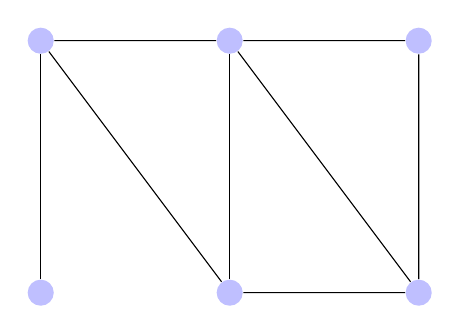
\begin{tikzpicture}
[scale=.8,auto=left,every node/.style={circle,fill=blue!25}]
  \node (n6) at (3,2) {};
  \node (n4) at (3,6) {};
  \node (n5) at (6,2) {};
  \node (n1) at (6,6) {};
  \node (n2) at (9,2) {};
  \node (n3) at (9,6) {};
  \foreach \from/\to in {n6/n4,n4/n5,n5/n1,n1/n2,n2/n5,n2/n3,n3/n1,n1/n4}
    \draw (\from) -- (\to);
\end{tikzpicture}
\caption{Et eksempel på en simpel, endelig graf} \label{simpel_graf}
\end{figure}


\noindent I Figur \ref{simpel_graf} er skitseret en simpel graf med $6$ knuder og $8$ forbindende kanter. \\ 

\noindent Optræder der et uordnet punktpar $\lbrace u,v \rbrace$ i grafen, som forbindes af to eller flere kanter, kaldes grafen en \textit{multigraf}, og findes der et punkt i grafen, som via en kant forbindes med sig selv (en \textit{løkke}), er der tale om en \textit{pseudograf}. Et eksempel kan ses nedenfor for de to grafer.

\begin{figure}[!htb]
   \begin{minipage}{0.48\textwidth}
     \centering
     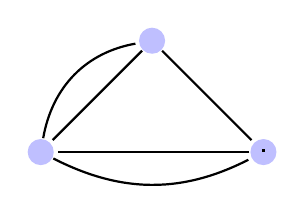
\begin{tikzpicture}[shorten >=1pt,auto,node distance=2cm,
                thick,main node/.style={circle,fill=blue!25}]

  \node[main node] (a) {};
  \node[main node] (b) [below left of=a] {};
  \node[main node] (c) [below right of=a] {};

  \path
    (a) edge node {} (b)
        edge node {} (c)
    (b) edge [bend left=35] node {} (a)
        edge [bend right=27] node {} (c)
    (c) edge [] node {} (c)
        edge node [] {} (b);

\end{tikzpicture}
     \caption{Eksempel på en multigraf}\label{Fig:Data1}
   \end{minipage}\hfill
   \begin{minipage}{0.48\textwidth}
     \centering
     \tikzset{every loop/.style={}}

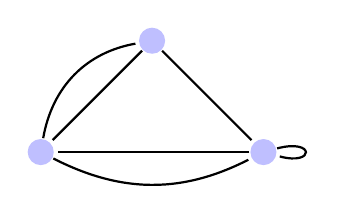
\begin{tikzpicture}[shorten >=1pt,auto,node distance=2cm,
                thick,main node/.style={circle,fill=blue!25}]

  \node[main node] (a) {};
  \node[main node] (b) [below left of=a] {};
  \node[main node] (c) [below right of=a] {};

  \path
    (a) edge node {} (b)
        edge node {} (c)
    (b) edge [bend left=35] node {} (a)
        edge [bend right=27] node {} (c)
    (c) edge [loop right] node {} (c)
        edge node [above] {} (b);
\end{tikzpicture}



     \caption{Eksempel på en pseudograf}\label{Fig:Data2}
   \end{minipage}
\end{figure}


\noindent Det kan imidlertid være nødvendigt at give kanterne retning, for at indikere, hvilken retning forbindelsen mellem to punkter har. I grafer over eksempelvis trafikale netværk, kan det være nødvendigt at indikere, i hvilken retning, trafikken kører eller at angive ensrettede strækninger. Til disse formål vil en simpel graf være utilstrækkelig idet kanterne deri netop ingen bestemt retning har. Derfor anledes Definition \ref{def_retn_graf} 
af en \textit{orienteret graf}:

\begin{defn}
En orienteret graf $G = (V, E)$ består af en mængde knuder, $V$, og en mængde \textit{orienterede} kanter, $E$, hvorom der gælder, at $V, E \neq \emptyset$.\\
En orienteret kant kan opfattes som et ordnet punktpar $(u,v), u,v \in  V$.
\label{def_retn_graf}
\end{defn} 

\noindent Definition \ref{def_retn_graf} tillader ydermere muligheden for, at et knudepar kan forbindes af indtil flere orienterede kanter. Findes dette i grafen, kaldes den en \textit{oritenteret multigraf}, og denne må også indeholde løkker. I det tilfælde, at alle knudepar kun forbindes af netop én ortienteret kant, og der ingen løkker er, er grafen en \textit{simpel orienteret graf}.

\noindent Det kan imidlertid være nødendigt at give kanterne retning for at indikere, hvilken retning forbindelsen mellem to punkter har. I grafer over eksempelvis trafikale netværk, kan det være nødvendigt at indikere i hvilken retning, trafikken kører, eller at angive ensrettede strækninger. Til disse formål vil en simpel graf være utilstrækkelig, idet kanterne deri netop ingen bestemt retning har. Derfor anledes definition \ref{def_retn_graf} 
af en \textit{retningsbestemt graf}:

\begin{defn}
En retningsbestemt graf $G = (V, E)$ består af et antal knuder, $V$, og et antal \textit{retningsbestemte} kanter, hvorom der gælder, at $V, E \neq \emptyset$.\\
En retningsbestemt kant $(u,v)$ forbinder et knudepar, så at kanten starter i $u$ og ender i $v$.
\label{def_retn_graf}
\end{defn} 

\noindent Denne definition (\ref{def_retn_graf}) tillader ydermere muligheden for, at et knudepar kan forbindes af indtil flere retningsbestemte kanter. Findes dette i grafen, kaldes den en \textit{retningsbestemt multigraf}, og denne må også indeholde løkker. I det tilfælde at alle knudepar kun forbindes af netop én retningsbestemt kant, er grafen en \textit{simpel retningsbestemt graf}.


\begin{figure}[h]
\centering
	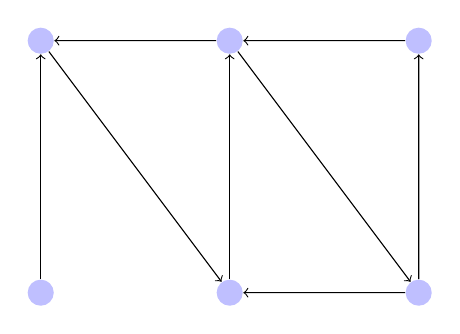
\begin{tikzpicture}
	[scale=.8,auto=left,every node/.style={circle,fill=blue!25}]
  \node (n6) at (3,2) {};
  \node (n4) at (3,6) {};
  \node (n5) at (6,2) {};
  \node (n1) at (6,6) {};
  \node (n2) at (9,2) {};
  \node (n3) at (9,6) {};
  \foreach \from/\to in {n6/n4,n4/n5,n5/n1,n1/n2,n2/n5,n2/n3,n3/n1,n1/n4}
    \draw [->] (\from) -- (\to);
	\end{tikzpicture}
\caption{Et eksempel på en retningsbestemt graf, hvor man kan se pilene definere retningen.}
\end{figure}

\noindent Eksempelvis er der i et netværk af computere, som er forbundet til hinanden, brug for at kommunikation kan ske både frem og tilbage mellem enhederne. Derfor er et simpelt orienteret system ikke nok da det netop kræves at der kan forekomme flere interaktioner mellem forskellige computere. Til dette skal man bruge orienterede multigrafer.
=======
\noindent Et simpelt retningsbestemt system er dog ikke nok i et computernetværk, som kræver, at der kan forekomme flere interaktioner mellem forskellige computere. Til dette skal man bruge orienterede multigrafer.


\begin{figure}[h]
\centering
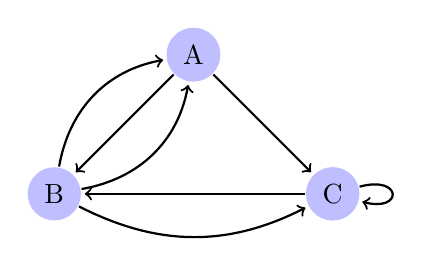
\begin{tikzpicture}[->,shorten >=1pt,auto,node distance=2.5cm,
                thick,main node/.style={circle,fill=blue!25}]

  \node[main node] (a) {A};
  \node[main node] (b) [below left of=a] {B};
  \node[main node] (c) [below right of=a] {C};

  \path
    (a) edge node {} (b)
        edge node {} (c)
    (b) edge [bend left=35] node {} (a)
    	    edge [bend right=35] node {} (a)
        edge [bend right=27] node {} (c)
    (c) edge [loop right] node {} (c)
        edge node [above] {} (b);
    (a) edge [bend right=30] node {} (b)
\end{tikzpicture}
\caption{Her kan man se et eksempel på en orienteret multigraf, hvor der både er adskillige kanter mellem knuderne A og B, samt er der en løkke tilstede i knudepunktet C }
\end{figure}


\noindent Nogle gange er det nødvendigt at konstruere og arbejde med computernetværker som både kan arbejde begge veje, samt ensrettet. Til dette bruger man kombineret grafer, som både indholder orienteret og ikke-orienteret kanter. Disse grafer kaldes \textit{kombinerede grafer}.
=======
\noindent Nogle gange er det nødvendigt at konstruere og arbejde med computernetværker, som både kan arbejde begge veje samt ensrettet. Til dette bruger man kombinerede grafer, som både indholder orienterede og ikke-orienterede kanter. Disse grafer kaldes kombinerede grafer.


\begin{figure}[!h]
\centering
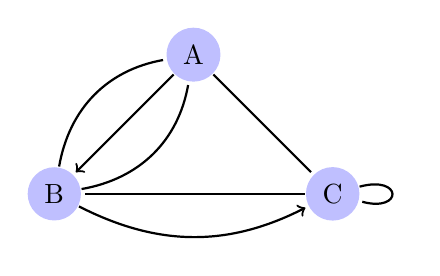
\begin{tikzpicture}[shorten >=1pt,auto,node distance=2.5cm,
                thick,main node/.style={circle,fill=blue!25}]

  \node[main node] (a) {A};
  \node[main node] (b) [below left of=a] {B};
  \node[main node] (c) [below right of=a] {C};

    \path [->] (a) edge node {} (b);
    \path      (a) edge node {} (c);
    \path      (b) edge [bend left=35] node {} (a);
    	\path      (b) edge [bend right=35] node {} (a);
    \path [->] (b) edge [bend right=27] node {} (c);
    \path      (c) edge [loop right] node {} (c);
    \path      (c) edge node [above] {} (b);
\end{tikzpicture}
\caption{Her kan en kombineret graf ses, hvor den både indeholder orienterede og ikke-orienterede kanter, samt indeholder en løkke i knudepunktet C}
\end{figure}

\noindent For at kunne danne et større overblik over de forskellige grafer og deres defination og karakteristika , er Tabel 5.1 konstrueret.

\begin{table}[h]
\begin{tabular}{|c|c|c|c|}
\hline 
Type & Kanter & Flerdobbelte kanter tilladt & Løkker \\ 
\hline
Simpel graf & Ikke-orienteret & Nej & Nej	 \\ 

Multigraf & Ikke-orienteret & Ja & Nej \\ 

Pseudograf & Ikke-orienteret & Ja & Ja \\ 
 
Simpel orienteret graf & Orienteret & Nej & Nej \\ 
 
Orienteret multigraf & Orienteret & Ja & Ja \\ 
 
Kombineret graf & Orienteret og ikke-orienteret & Ja & Ja \\ 
\hline 
\end{tabular}
\caption{Her kan der ses et overblik over de forskellige grafer} \label{table:graf_oversigt}
\end{table}

\usetikzlibrary{arrows, positioning}
\section{Grafer 2}
\subsection{Grafterminologi}

Der findes begreber til at beskrive kanter og knuder i ikke-orienterede grafer, som bl.a. beskriver hvordan knuder og kanter er orienterede i forhold til hinanden samt hvor mange knuder eller kanter, der er forbundet til en given knude.

\begin{defn}
To knuder $u$ og $v$ siges at være naboer i en ikke-orienteret graf $G$, hvis $u$ og $v$ er endepunkter i en kant $e$. Desuden siges kanten $e$ at forbinde $u$ og $v$, og $e$ er incident med både $u$ og $v$.
\end{defn}

\begin{defn}
En mængde af alle naboer til en knude $v$ i en graf $G=(V,E)$ betegnes $N(v)$ og kaldes et nabolag af $v$. Hvis $A$ er en delmængde af $V$, betegner $N(A)$ mængden af alle knuder i $G$, som er nabo til mindst én knude i $A$.
\end{defn}

\begin{defn}
Graden af en knude i en ikke-orienteret graf betegnes $deg(v)$ og er antallet af kanter incidente med den givne knude.  Et muligt loop vil bidrage med to grader til knuden. 
\end{defn}

En knude med grad 0 betegnes som værende \textit{isoleret} og har ingen incidente kanter. En knude med grad 1 betegnes som et \textit{vedhæng} og har netop én incident kant.

\begin{exmp}
Bestem graden af knuderne og nabolagene for knuderne i grafen i figur \ref{eksempel_nabo} og identificer isolerede knuder eller vedhæng.\\
Graden af en knude i grafen i figur \ref{eksempel_nabo} bestemmes ved at identificere antal incidente kanter til knuden. Derfor er $deg(A)=1$, $deg(B)=3$, $deg(C)=3$, $deg(D)=4$, $deg(E)=3$ og $deg(F)=2$. 
Nabolagene for de enkelte knuder er mængden af naboknuder. 
Derfor er $N(A)=\lbrace B \rbrace$, $N(B)=\lbrace A, C, D \rbrace$, $N(C)=\lbrace B, D, E \rbrace$, $N(D)=\lbrace B, C, E, F \rbrace$, $N(E)=\lbrace C, D, F \rbrace$ og $N(F)=\lbrace D, E \rbrace$. 
I grafen er A et vedhæng, og der forefindes ingen isolerede knuder.
\end{exmp}

\begin{figure}[h]
\centering
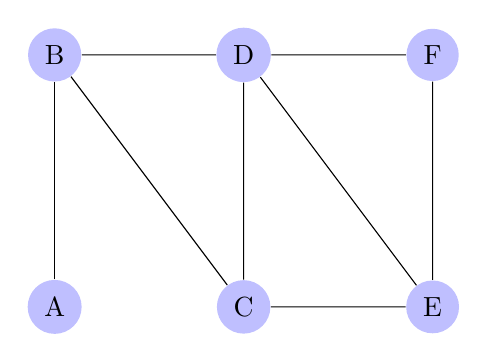
\begin{tikzpicture}
[scale=.8,auto=left,every node/.style={circle,fill=blue!25}]
  \node (n6) at (3,2) {A};
  \node (n4) at (3,6) {B};
  \node (n5) at (6,2) {C};
  \node (n1) at (6,6) {D};
  \node (n2) at (9,2) {E};
  \node (n3) at (9,6) {F};
  \foreach \from/\to in {n6/n4,n4/n5,n5/n1,n1/n2,n2/n5,n2/n3,n3/n1,n1/n4}
    \draw (\from) -- (\to);
\end{tikzpicture}
\caption{Simpel ikke-orienteret graf} \label{eksempel_nabo}
\end{figure}

For at beskrive summen af graderne for alle knuder i en graf anvendes \textit{The Handshaking Theorem}. 

\begin{thm}\label{handshake}
\textbf{The Handshaking Theorem}. Lad $G=(V,E)$ være en ikke-orienteret graf med $m$ kanter. Så er summen af knudernes grader \\
\begin{align*}
2m=\sum_{v \in V}deg(v)
\end{align*}
\end{thm}

\begin{proof}
I en ikke-orienteret graf med $m$ kanter, bidrager hver kant i en graf med to grader - én grad til hvert endepunkt. Det samlede antal grader for alle knuder i en graf stiger således med to pr. kant og summen af $deg(v)$ er $2m$. 
\end{proof}

Som følge af \ref{handshake} er summen af knudernes grader et lige tal. Derfor har en ikke-orienteret graf et lige antal knuder, hvor graden er et ulige tal.

\begin{thm}
En ikke-orienteret graf har et lige antal knuder af ulige grad. 
\end{thm}

\begin{proof}
Lad $V_1$ og $V_2$ være henholdsvis mængden af knuder af lige grad og mængden af knuder af ulige grad i en ikke-orienteret graf $G=(V,E)$ med $m$ kanter. Så er \\
\begin{align*}
2m=\sum_{v \in V}deg(v)=\sum_{v \in V_1}deg(v)+ \sum_{v \in V_2}deg(v)
\end{align*}
Da $deg(v)$ er lige for $v \in V_1$, er summen $\sum_{v \in V_1}deg(v)$ også lige. Summen af de to led på højresiden i ligningen er lige, fordi de tilsammen er lig $2m$, hvorfor $\sum_{v \in V_2}deg(v)$ også er lige. Summen $\sum_{v \in V_2}deg(v)$ består af en række ulige tal, og for at summen bliver lige, skal der således være et lige antal ulige led i summen.
Idet summen af graderne for knuderne af ulige grad i grafen er lige, må der være et lige antal af sådanne knuder.
\end{proof}




\subsection{Repræsentation af grafer}

Der er flere brugbare måder at repræsentere grafer på, og man ønsker i hvert tilfælde at vælge den pæneste repræsentation. \\
En overskuelig måde at repræsentere en graf på er ved matricer. To matricer, der almindeligvis bruges, er nabo-matricer, der er baseret på nabo-knuder, og incidens-matricer baseret på incidensen af knuder og kanter. \\
Antag at $G=(V,E)$ er en simpel graf med $n$ knuder, hvor knuderne i $G$ står skrevet i vilkårlig rækkefølge som $v_1$, $v_2$, \dots , $v_n$. Nabo-matricen $A$  af G er en $n \times n$ nul-et matrix, med 1 som den $(i,j)$’te indgang når $v_i$ og $v_j$ er naboer, og 0 er den $(i,j)$’te indgang, når de ikke er naboer. Hvis nabo-matricen er $A=[a_{ij}]$ så er

\begin{align*}
a_{ij}= \left\{\begin{array}{cc}
1 & \textrm{hvis} \  \lbrace v_i, v_j \rbrace \  \textrm{er} \  \textrm{en} \  \textrm{kant} \  \textrm{i} \  G \\
0 & \textrm{ellers} \\
\end{array}\right.
.
\end{align*}

En nabo-matrix af en graf er baseret på den valgte ordning af knuderne, hvorfor der kan være $n!$ forskellige nabo-matricer for en graf med $n$ knuder, idet der er $n!$ forskellige måder at ordne de $n$ knuder. Nabo-matricen for en simpel graf er symmetrisk dvs. $a_{ij}=a_{ji}$, da begge indgange er 1, når de relaterede knuder er naboer, og 0 hvis de ikke er. Da en simpel graf ikke består af loops, er hver indgang $a_{ii},i=1,2,3, \dots ,n$ $0$. \\
Nabo-matricer kan også bruges til at repræsentere ikke-orienterede grafer med loops og flere kanter til samme knuder. Et loop ved en knude $v_i$ er repræsenteret ved 1 ved position $(i,i)$ i nabo-matricen. Når flere kanter forbinder det samme par af knuder $v_i$ og $v_j$, eller der er flere loops ved samme knude til stede, er nabo-matricen ikke længere en nul-et matrix, i det den $(i,j)$’te indgang af matricen er lig antallet af kanter forbundet til ${v_i,v_j}$. Alle ikke-orienterede grafer, herunder multi- og pseudografer, har symmetriske nabo-matricer. 

 \begin{equation*}
  \mathbf{A}=
  \begin{blockarray}{*{6}{c} l}
    \begin{block}{*{6}{>{$\footnotesize}c<{$}} l}
      A & B & C & D & E & F \\
    \end{block}
    \begin{block}{[*{6}{c}]>{$\footnotesize}l<{$}}
      0 & 1 & 0 & 0 & 0 & 0 \bigstrut[t]& A \\
      1 & 0 & 1 & 1 & 0 & 0 \bigstrut[t]&B \\
      0 & 1 & 0 & 1 & 1 & 0 \bigstrut[t]&C \\
      0 & 1 & 1 & 0 & 1 & 1 \bigstrut[t]& D \\
      0 & 0 & 1 & 1 & 0 & 1 \bigstrut[t]& E \\
      0 & 0 & 0 & 1 & 1 & 0 \bigstrut[t]& F \\
    \end{block}
  \end{blockarray}
\end{equation*}

\noindent En anden almindelig måde at repræsentere grafer på er ved incidens-matricer. Lad $G=(V,E)$ være en ikke-orienteret graf med knuderne $v_1$, $v_2$, \dots , $v_n$ og kanterne $e_1$, $e_2$, \dots , $e_n$. Incidens-matricen, i forhold til ordningen af $V$ og $E$, er en $n x m$ matrix $M=[m_{ij}]$, hvor 
\begin{align*}
m_{ij}= \left\{\begin{array}{cc}
1 & \textrm{hvis} \  {e_j} \  \textrm{er} \  \textrm{nabo} \ \textrm{til} \ v_i \\
0 & \textrm{ellers} \\
\end{array}\right.
\end{align*}

\noindent Incidensmatricer kan også bruges til at repræsentere flere kanter og løkker. Flere kanter ved én knude er repræsenteret i incidens-matricen ved kolonner med identiske indgange, idet disse kanter er incidente med det samme knudepar. Løkker er repræsenteret ved en kolonne med præcis én indgang lig 1, der svarer til den knude, der er incident med løkken. 

 \begin{equation*}
  \mathbf{M}=
  \begin{blockarray}{*{8}{c} l}
    \begin{block}{*{8}{>{$\footnotesize}c<{$}} l}
      1 & 2 & 3 & 4 & 5 & 6 & 7 & 8 \\
    \end{block}
    \begin{block}{[*{8}{c}]>{$\footnotesize}l<{$}}
      1 & 0 & 0 & 0 & 0 & 0 & 0 & 0 \bigstrut[t]& A \\
      1 & 1 & 1 & 0 & 0 & 0 & 0 & 0 \bigstrut[t]&B \\
      0 & 1 & 0 & 1 & 1 & 0 & 0 & 0 \bigstrut[t]&C \\
     0 & 0 & 1 & 1 & 0 & 1 & 1 & 0 \bigstrut[t]& D \\
      0 & 0 & 0 & 0 & 1 & 1 & 0 & 1 \bigstrut[t]& E \\
     0 & 0 & 0 & 0 & 0 & 0 & 1 & 1 \bigstrut[t]& F \\
    \end{block}
  \end{blockarray}
\end{equation*}


\begin{figure}[!h]
  \centering
  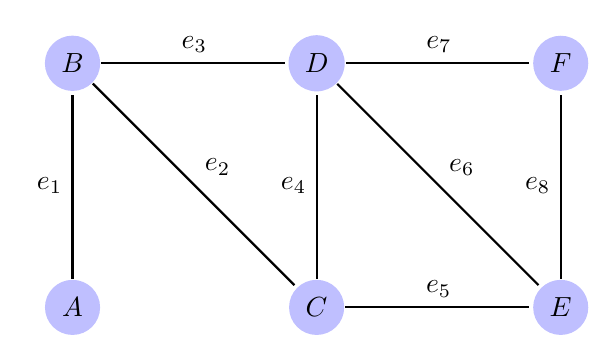
\begin{tikzpicture}
  [shorten >=1pt,node distance=3.1cm,on grid,auto]
    \tikzstyle{state}=[shape=circle,fill=blue!25,thick,minimum size=0.7cm]

    \node[state] (A) {$A$};
    \node[state,above of=A] (B) {$B$};
    \node[state,right of=A] (C) {$C$};
    \node[state,right of=B] (D) {$D$};
    \node[state,right of=C] (E) {$E$};
    \node[state,right of=D] (F) {$F$};

    \path[-,draw,thick]
    (A) edge node {$e_1$} (B)
    (B) edge node {$e_2$} (C)
    (B) edge node {$e_3$} (D)
    (C) edge node {$e_4$} (D)
    (C) edge node {$e_5$} (E)
    (D) edge node {$e_6$} (E)
    (D) edge node {$e_7$} (F)
    (E) edge node {$e_8$} (F)
    ;
  \end{tikzpicture}
  \caption{Model}
  \label{fig:f1}
\end{figure}





Flere problemstillinger kan modelleres ved brug af grafer med vægte tildelt kanterne. 
Det kan f.eks. være distance, den samlede rejsetid, eller billetprisen for at rejse mellem to byer. 
Grafer, der har vægte tildelt kanterne, kaldes vægtede grafer. 
Der opstår jævnligt forskellige typer af problemer, der involverer vægtede grafer, hvor en korteste rute, mellem to knuder i et netværk, skal bestemmes. 
Længden af en vej i en graf uden vægte er tidligere betegnet ved antallet af kanter, vejen går igennem.
I en vægtet graf er længden af vejen summen af alle kanternes vægte, der indgår i vejen. 
Et interessant problem, som involverer vægtede grafer, søger en kreds af kortest mulig totallængde, der besøger hver knude i en komplet graf præcis én gang.
Der er her tale om \emph{traveling salesperson problem}, som søger dén rækkefølge, knuderne skal besøges i, som resulterer i en kreds af kortest mulig længde. 

\section{Komplette grafer}
En komplet graf er en graf hvor et hvert unikt par af knuder i grafen er forbundet.
En komplet graf navngives $K_n$ hvor $n$ er antallet af knuderf i grafen.
I figur \ref{fig:komplette_grafer} ses de første 5 komplette grafer.
En graf hvor mindst ét par af knuder ikke er forbundet, kaldes en ikke-komplet graf.

\begin{figure}[h]
	\centering
	% Radius of regular polygons
\newdimen\R
\R=1cm

\begin{tikzpicture}[thick]
  \foreach \x in {1,2,3,4,5}{
    \node[yshift=-1.5\R, xshift=\x*2.5\R-2.5\R] {$K_\x $} {};
  }
  \begin{scope}[every node/.style={circle,fill=blue!25}]
    \node (0:0) {};

    \foreach \x in {1,2}{
      \node[xshift=2.5\R] (\x) at (\x*180-180:\R) {};
    }
    \path (1) edge (2);

    \foreach \x in {1,2,3}{
      \node[xshift=5\R] (\x) at (\x*120-120:\R) {};
    }
    \path (1) edge (2);
    \path (2) edge (3);
    \path (3) edge (1);
  
    \foreach \x in {1,2,3,4}{
      \node[xshift=7.5\R] (\x) at (\x*90-90:\R) {};
    }
    \foreach \x in {1,2,3}{
      \path (4) edge (\x);
    }
    \foreach \x in {1,2}{
      \path (3) edge (\x);
    }
    \path (1) edge (2);
  
    \foreach \x in {1,2,3,4,5}{
      \node[xshift=10\R] (\x) at (\x*72-72:\R) {};
    }
    \foreach \x in {1,2,3,4}{
      \path (5) edge (\x);
    }
    \foreach \x in {1,2,3}{
      \path (4) edge (\x);
    }
    \foreach \x in {1,2}{
      \path (3) edge (\x);
    }
    \path (1) edge (2);
  \end{scope}
\end{tikzpicture}

	\caption{De første $5$ komplette grafer} \label{fig:komplette_grafer}
\end{figure}

Antallet af kanter i en komplet graf $K_n$ afhænger kun af $n$.

\begin{thm}
	For en komplet graf $K_n = (V_n, E_n)$ med $n$ knuder er $|E_n|$ antallet af kanter. Da er
	\begin{align*}
		|E_n| = \frac{n (n - 1)}{2}
	\end{align*}
\end{thm}
\begin{proof}
	For at gennemføre et induktionsbevis skal basisskridtet og induktionsskridtet gennemføres.
	Lad propositionen $P(n)$ være at $|E_n|= \frac{n (n - 1)}{2}$, hvor $n$ er antal knuder i en komplet graf $K_n$ og $m$ være antal kanter.

	\textit{Basisskridt:} $K_1$ består af en enkelt knude, og da der ikke er et par af knuder i grafen, må der da ikke eksistere nogen kanter.
	$\frac{ 1 \cdot 0}{2} = 0$, hvilket betyder at $P(1)$ er sand. Da er basisskidtet gennemført.

	\textit{Induktionsskridt:} Det skal nu vises at der for et vilkårligt $k$ gælder at $P(k) \to P(k + 1)$, altså at $|E_k| = \frac{k (k - 1)}{2}$ medfører at $|E_{k+1}| = \frac{k (k + 1)}{2}$.

	Antag at $|E_k| = \frac{k (k - 1)}{2}$ for $K_k$.
	Den næste komplette graf $K_{k+1}$ må være den graf hvor der er én til knude. Denne nye knude $v$ skal være forbundet til alle knuder i $K_k$ for at være en komplet graf. $\deg (v)$ må da være lig $k$. Da må
	\begin{align*}
		|E_{k+1}| 
		&= |E_k| + k \\
		&= \frac{k (k - 1)}{2} + k \\
		&= \frac{k^2 - k}{2} + \frac{2k}{2} \\
		&= \frac{k^2 + k}{2} \\
		&= \frac{k (k + 1)}{2}
	\end{align*}
	Dette er netop $P(k + 1)$, hvilket betyder at induktionsskridtet er gennemført.
\end{proof}


\section{Parring i grafer}
Nogle grafer har den egenskab, at deres knuder kan deles op i to undergrupper, således at knuder fra dan samme undergruppe ikke forbindes af kanter, men kun forbindes med knuder fra den anden undergruppe.
Dette kaldes parring i grafer.
Parring i grafer kan blandt andet bruges til at vise relationer mellem to forskellige typer objekter.
Et eksempel på dette kan være en graf, der viser hvilke studerende der tager hvilke kurser, så de studerende er i en undergruppe og kurserne i en anden. 

\begin{defn}
En simpel graf $G$ kaldes parret, hvis dens knuder kan deles op i to adskilte undergrupper $V_1$ og $V_2$, så hver kant i grafen forbinder en knude fra $v_1$ og $V_2$, men ikke to knuder fra den samme undergruppe.
Når dette gælder, kaldes parret ($V_1,V_2$) en parring af $V$ i $G$.
\end{defn}

\begin{exmp}
I Figur \ref{parret_graf} ses en parret graf, med de to undergrupper ($v1,v2,v3$) og ($v3,v4$). 
På grafen ses det, at hvert kant forbinder en knude fra den ene undergruppe med en fra den anden, mens ingen kanter forbinder to knuder fra den samme undergruppe. 
Deruder ses det også, at der ikke er en kant fra alle knuder i en gruppe til alle knuder i den anden undergruppe.
Der er for eksempel ikke en kant mellem $v3$ og $v5$. 
Der behøver ikke være kanter fra alle knuder i den ene undergruppe til den anden for at grafen er parret.
Havde der været en kant mellem $v1$ og $v2$ havde grafen ikke været parret, da der ikke må være en kant mellem to knuder fra samme undergruppe.
\end{exmp}

\begin{figure}
\centering
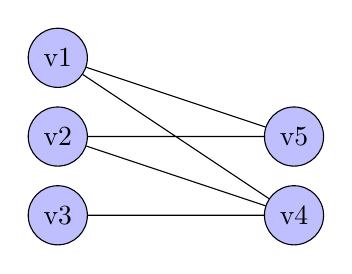
\begin{tikzpicture}[every node/.style={draw,shape=circle,fill=blue!25}]
\path (-1.5,0) node (p0) {v1}
(-1.5,-1) node (p1) {v2}
(-1.5,-2) node (p2) {v3}
(1.5,-2) node (p3) {v4}
(1.5,-1) node (p4) {v5};
\draw 
(p0) -- (p3)
(p0) -- (p4)
(p1) -- (p3)
(p1) -- (p4)
(p2) -- (p3);
\end{tikzpicture}
\caption{Parret graf}
\label{parret_graf}
\end{figure}

\begin{thm}
En simpel graf er parret hvis og kun hvis, det er mulig at tildele hver knude en af to farver, således at hver kant ikke forbinder to knuder af samme farve. 
\label{farve_satning}
\end{thm}

\begin{proof}
Antag at $G=(V,E)$ er en parret simpel graf. Så er $V=V_1 \cup V_2$, hvor $V_1 \cap V_2 = Ø$ og hver kant i E forbinder en knude i $V_1$ med en knude i $V_2$. 
Tildeles en farve til alle knuder i $V_1$ og en anden farve til alle knuderne i $V_2$, så vil ingen kanter forbinde to knuder af samme farve. 
Gå så ud fra, at det er muligt at tildele farver til knuder, hvor der kun bruges to farver, hvor hvert knudepar består af to knuder af hver sin farve.
Når det gælder er $V_1 \cap V_2=Ø$ og $V=V_1 \cup V_2$.
Ydermere forbinder hver kant en knude i $V_1$ til en knude i $V_2$, da ingen naboknuder kan tilhøre samme undergruppe. 
\end{proof}

\begin{exmp}
I Figur \ref{farve_graf} ses en parret graf, hvor hver knude er tildelt en farve jævnfør sætning \ref{farve_satning}. 
Her ses det, hvordan hevr kant forbinder en rød knude med en blå knude, samt hvordan ingen kant forbinder to røde eller to blå knuder.

\begin{figure}[h]
\centering
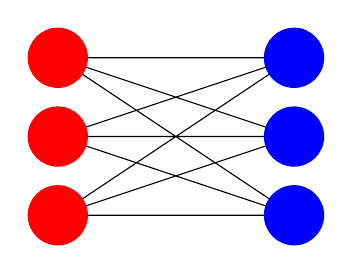
\begin{tikzpicture}[every node/.style={draw,shape=circle,fill=blue!25}]
\path (-1.5,0) node (p0) [red]{v1}
(-1.5,-1) node (p1) [red]{v2}
(-1.5,-2) node (p2) [red]{v3}
(1.5,-2) node (p3) [blue]{v4}
(1.5,-1) node (p4) [blue]{v5}
(1.5,0) node (p5) [blue]{v6};
\draw 
(p0) -- (p3)
(p0) -- (p4)
(p1) -- (p3)
(p1) -- (p4)
(p2) -- (p3)
(p2) -- (p4)
(p5) -- (p0)
(p5) -- (p1)
(p5) -- (p2);
\end{tikzpicture}
\caption{Farveopdelt parret graf}
\label{farve_graf}
\end{figure}
\end{exmp}

En parret graf kan siges at være komplet. 
At en graf er komplet betyder, at hver knude fra en undergruppe er forbundet med alle knuder fra den anden undergruppe. 
En sådan graf betegnes $K_m,n$, hvor m er antallet af knuder i den ene undergruppe og n antallet i den anden undergruppe. 

\begin{exmp}
Grafen i Figur \ref{farve_graf} er også en komplet parret graf, fordi hver rød knude er forbundet med hver blå knude. 
Denne graf kaldes derfor $K_{3,3}$
\end{exmp}

Det ønskes nu at undersøge, hvornår der eksisterer en komplet parring mellem to undergrupper i en graf. 
I følgende sætning opsættes nogle nødvendige kriterier, der beskriver hvornår en komplet parring eksisterer. 

\begin{thm}[Bla]
\textbf{Ægteskabs Sætning}
Den parrede graf $G=(V,E)$ med undergrupperne ($V_1,V_2$) har en komplet parring fra ,$V_1$ til $V_2$.
\end{thm}
